\RequirePackage{ifpdf}
%\documentclass[journal]{vgtc}                % final (journal style)
\documentclass[review,journal]{vgtc}         % review (journal style)
%\documentclass[widereview]{vgtc}             % wide-spaced review
%\documentclass[preprint,journal]{vgtc}       % preprint (journal style)
%\documentclass[electronic,journal]{vgtc}     % electronic version, journal

%% Uncomment one of the lines above depending on where your paper is
%% in the conference process. ``review'' and ``widereview'' are for review
%% submission, ``preprint'' is for pre-publication, and the final version
%% doesn't use a specific qualifier. Further, ``electronic'' includes
%% hyperreferences for more convenient online viewing.

%% Please use one of the ``review'' options in combination with the
%% assigned online id (see below) ONLY if your paper uses a double blind
%% review process. Some conferences, like IEEE Vis and InfoVis, have NOT
%% in the past.

%% Please note that the use of figures other than the optional teaser is not permitted on the first page
%% of the journal version.  Figures should begin on the second page and be
%% in CMYK or Grey scale format, otherwise, colour shifting may occur
%% during the printing process.  Papers submitted with figures other than the optional teaser on the
%% first page will be refused.
%\begin{figure}[htb]
%	\centering
%	\fbox{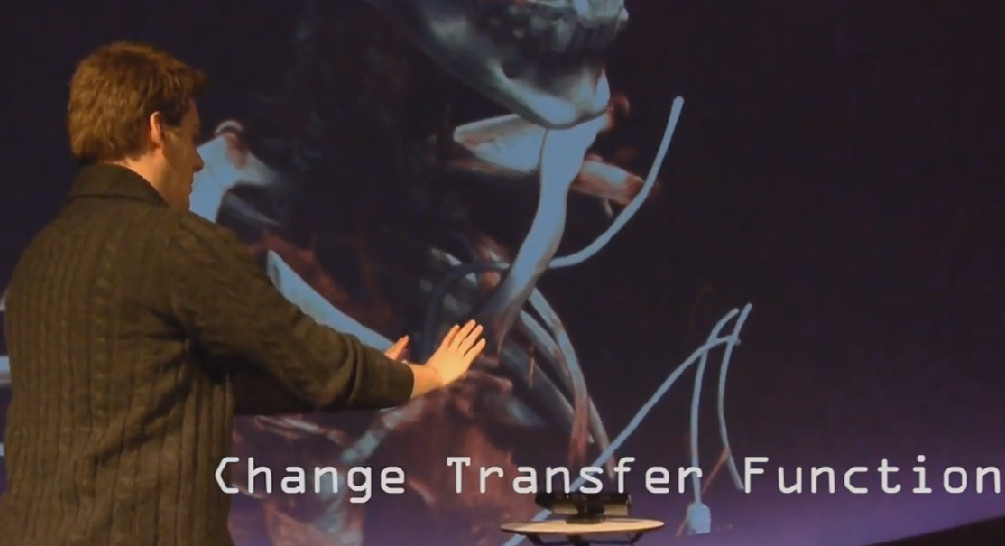
\includegraphics[width=1.0\linewidth]{images/dome_tf_change}}
%	\caption{Dome Closeup}
%	\label{img:dome_tf_change}
%\end{figure}

%% These three lines bring in essential packages: ``mathptmx'' for Type 1
%% typefaces, ``graphicx'' for inclusion of EPS figures. and ``times''
%% for proper handling of the times font family.

\usepackage{mathptmx}
\usepackage{graphicx}
\usepackage{times}
\usepackage{amsmath}
\usepackage{flushend}
\usepackage{subfigure}
\usepackage[noabbrev]{cleveref}
\usepackage{color}
%\usepackage[caption=false]{subfig}
\setlength{\fboxsep}{0pt}
\newcommand{\todo}[1]{\textbf{\textcolor{red}{[TODO: {#1}]}}}

%% We encourage the use of mathptmx for consistent usage of times font
%% throughout the proceedings. However, if you encounter conflicts
%% with other math-related packages, you may want to disable it.

%% This turns references into clickable hyperlinks.
%%\usepackage[bookmarks,backref=true,linkcolor=black]{hyperref} %,colorlinks
%%\hypersetup{
%%  pdfauthor = {},
%%  pdftitle = {},
%%  pdfsubject = {},
%%  pdfkeywords = {},
%%  colorlinks=true,
%%  linkcolor= black,
%%  citecolor= black,
%%  pageanchor=true,
%%  urlcolor = black,
%%  plainpages = false,
%%  linktocpage
%%}

%% If you are submitting a paper to a conference for review with a double
%% blind reviewing process, please replace the value ``0'' below with your
%% OnlineID. Otherwise, you may safely leave it at ``0''.
\onlineid{18}

%% declare the category of your paper, only shown in review mode
\vgtccategory{Position Paper}

%% allow for this line if you want the electronic option to work properly
\vgtcinsertpkg

%% In preprint mode you may define your own headline.
%\preprinttext{To appear in an IEEE VGTC sponsored conference.}

%% Paper title.

%\title{An Audience-centric View on Interaction Techniques \\for the Interactive Presentation of Scientific 3D Data}
\title{Interaction Techniques as a Communication Channel\\when Presenting 3D Visualizations} % Alternative

%% This is how authors are specified in the journal style

%% indicate IEEE Member or Student Member in form indicated below
%% indicate IEEE Member or Student Member in form indicated below
%\author{Erik Sund\'en, \textit{Member, IEEE}, Alexander Bock, \textit{Student Member, IEEE}, Daniel J\"onsson, \textit{Student Member, IEEE}\\ and Timo Ropinski, \textit{Member, IEEE}}
%\authorfooter{
%% insert punctuation at end of each item
%\item
% Erik Sund\'en, Alexander Bock, Daniel J\"onsson and Timo Ropinski are with Link{\"o}ping University. E-mail: \{erik.sunden,alexander.bock,daniel.jonsson,timo.ropinski\}@liu.se.
%}

\author{Erik Sund\'en\thanks{e-mail:erik.sunden@liu.se}\\ %
        \scriptsize Link{\"o}ping University %
\and Alexander Bock\thanks{e-mail:alexander.bock@liu.se}\\ %
			   \scriptsize Link{\"o}ping University %
\and Daniel J\"onsson\thanks{e-mail:daniel.jonsson@liu.se}\\ %
          \scriptsize Link{\"o}ping University %
\and Anders Ynnerman\thanks{e-mail:anders.ynnerman@liu.se}\\ %
          \scriptsize Link{\"o}ping University %
\and Timo Ropinski\thanks{e-mail:timo.ropinski@liu.se}\\ %
           \scriptsize Link{\"o}ping University }


%other entries to be set up for journal
%\shortauthortitle{Sund\'en \MakeLowercase{\textit{et al.}}: Hands-only 2D vs 3D interaction when exploring volume data}
%\shortauthortitle{Firstauthor \MakeLowercase{\textit{et al.}}: Paper Title}

%% Abstract section.
\abstract{ 
In this position paper we discuss the usage of various interaction technologies with focus on the presentations of 3D visualizations involving a presenter and an audience. While an interaction technique is commonly evaluated from a user perceptive, we want to shift the focus from a sole analysis of the naturalness and the ease-of-use for the user, to focus on how expressive and understandable the interaction technique is when witnessed by the audience.
The interaction process itself can be considered to be a communication channel and a more expressive interaction technique might make it easier for the audience to comprehend the presentation.
Thus, while some natural interaction techniques for interactive visualization are easy to perform by the presenter, they may be less beneficial when interacting with the visualization in front of (and for) an audience.
%We would, for instance, consider a gesture performed in mid air as more expressive then the usage of a conventional pointing device such as the mouse.
Our observations indicate that the suitability of an interaction technique as a communication channel is highly dependent on the setting in which the interaction takes place.
Therefore, we analyze different presentation scenarios in an exemplary fashion and discuss how beneficial and comprehensive the involved techniques are for the audience.
We argue that interaction techniques complement the visualization in an interactive presentation scenario as they also serve as an important communication channel, and should therefore also be observed from an audience perceptive rather than exclusively a user perspective. 
} % end of abstract

%% Keywords that describe your work. Will show as 'Index Terms' in journal
%% please capitalize first letter and insert punctuation after last keyword
\keywords{Interaction, audience, 2D and 3D user interfaces, direct touch, touchless, voice control.}

%% ACM Computing Classification System (CCS). 
%% See <http://www.acm.org/class/1998/> for details.
%% The ``\CCScat'' command takes four arguments.

%\CCScatlist{ % not used in journal version
%   \CCScat{I.3.7}{Computer Graphics}{Three-Dimensional Graphics and Realism}{Color, shading, shadowing, and texture}
%}

%% Uncomment below to include a teaser figure.
%  \teaser{
%  \centering
%  \includegraphics[width=16cm]{CypressView}
%  \caption{In the Clouds: Vancouver from Cypress Mountain.}
%  }

%% Uncomment below to disable the manuscript note
%\renewcommand{\manuscriptnotetxt}{}

%% Copyright space is enabled by default as required by guidelines.
%% It is disabled by the 'review' option or via the following command:
% \nocopyrightspace

%%%%%%%%%%%%%%%%%%%%%%%%%%%%%%%%%%%%%%%%%%%%%%%%%%%%%%%%%%%%%%%%
%%%%%%%%%%%%%%%%%%%%%% START OF THE PAPER %%%%%%%%%%%%%%%%%%%%%%
%%%%%%%%%%%%%%%%%%%%%%%%%%%%%%%%%%%%%%%%%%%%%%%%%%%%%%%%%%%%%%%%%

\begin{document}

\maketitle

\section{Introduction}\label{sec:introduction}
Oral presentations, being the most traditional form of presentation techniques, have been around since time immemorial.
While they were initially limited to a lecturer talking, tools and techniques have been added to enhance the presentation.
A prime example of an enhancement, which shows that interaction techniques matter a great deal, is medical schools' education based on the dissection of cadavers in class.
Here, not only the presented content is of interest but also the way the lecturer interacts with the cadaver.

In recent years, different types of interaction have become increasingly common when presenting visualizations due to the introduction of low-cost interaction devices.
This change the fact that mouse and keyboard is not the paradigm used as the main type of interaction in all kinds of scenarios and allows us to analyze how interactions affect a presentation.
Touch screens are now the de-facto standard for handheld devices, supporting multi-touch interfaces for 2D gestures such as pinch or swipe, while low-cost solutions for touchless interaction, such as the Kinect or Leap Motion, even support 3D whole-body interaction interfaces \cite{978-0-85729-432-6, Shoemaker:2010:BIT:1868914.1868967}. 
These interaction interfaces have inspired a range of applications within interactive visualization~\cite{zora82163, Jalaliniya:2013:TIM:2494091.2497332, OHaraGSPVMCCRDC14, 0724-4983}.
The focus in research has been placed on the user's interaction expertise to determine if a type of interaction is suitable for a certain scenario within interactive visualization~\cite{5693835, so64840, DBLP:journals/tvcg/YiKSJ07}.
Yet, there has not been much attention on the fact that the interaction is also part of the presentation and therefore affects the audience.
As exemplified in the dissection example, if the audience can infer what will happen by witnessing the interaction, there is a significant impact on their understanding of the presentation.

We can draw an analogy to the field of visualization which generally separates the use of visualization into exploration, analysis and presentation steps, applying different approaches, tools and techniques for each step.
While the exploration phase requires a flexible interaction method, the presentation phase is usually limited to a few predetermined parameters.
The interface designer controls what can be viewed and, thus, makes the visualization more understandable for the audience.
The distinction between interaction techniques used for exploration as compared to presentation has, to our knowledge, not been considered and we will focus on interaction techniques for presentation purposes in the presence of a, possibly non-expert, audience.

Important parameters for measuring \emph{"good"} interaction techniques, with regard to communication with people, are how expressive~\cite{Brewster:2009:MIE:2227763.2227769} and natural~\cite{O'hara:2013:NTP:2442106.2442111} the gestures and speech are.
While many studies focus on analyzing these aspects for interaction by user or group of users~\cite{978-3-642-12552-2, Caridakis:2013:NIE:2504335.2504378}, we argue that they also play a significant role when observed by the audience during the presenters interaction with a visualization which happens in front of, and for, the audience.
Apart from controlling a visualization, the expressivity and naturalness of gestures also influence the knowledge transfer from the presenter to the audience. Thus, a 3D user interaction interface might be more preferable then a 2D user interaction interface, even if the 3D interface is more complex for the user, as it might be more expressive and natural for the audience to perceive.

We argue that the suitability and expressivity of a specific interaction method depends significantly on the screen sizes and the audience sizes.
We will therefore utilize scenarios from our experience that involve one person interacting with a visualization in order to present information to a, in general non-expert, audience (see Section~\ref{sec:scenario}).
The scenarios cover different situations with varying audience sizes and show the resulting constraints on the interaction design.

Based on these scenarios, we derive classes of interaction techniques and investigate their attributes related to suitability for the audience (see Section~\ref{sec:techniques}).
We will make the classification device-agnostic, as differences in the fundamental principles between many interaction devices in the same class are small.
For each class the applicability and usefulness for different audience sizes is investigated and discussed.
Section~\ref{sec:classification} reevaluates the presented scenarios in the same framework and connects the scenarios with the derived classes.

%
%
%
\section{Scenarios} \label{sec:scenario}
The scenarios described in this section are drawn from our experience in presenting scientific data to audiences of varying sizes and expertises.
We do not claim to cover all possible presentation cases in this section, yet we selected a subset of scenarios that cover a large variety of situations.

%
%
\subsection{Presentations using a Workstation} \label{sec:workstation}
In this scenario, the presentation is performed on a small screen, either handheld or a desktop monitor, and the audience usually consists of a single person or a small group.
As this setup will be most familiar to readers, we keep the description of this section concise.
The distance between the audience and the presenter is typically small and allows for a close communication.
The audience can easily communicate preferences in what to explore and may, in some cases, even intervene with the presenter to interact with the visualization.

An intuitive interaction can therefore engage the audience and create a more dynamic presentation.
An example can be seen in Figure~\ref{img:touch_workstation}, where the presenter uses a touch screen or touchpad to interact with an ultrasound scan of a fetus.
The standard interaction mode are camera interactions, where rotation, translation and zoom is controlled with single finger touch or multiple finger gestures interpreted in 2D.
The presenter can, in this case, switch to different modes to control other aspects of the visualization. For instance, another mode will change the interpretation of the single finger touch such that the threshold and opacity of the mapping between data and colors is changed according to the horizontal and vertical movement.
%Furthermore, as the display size is only 15\,'', one hand finger gestures are sufficient for all interaction possibilities.

%This scenario deals with small screens and 
%User-centered...
%
%Mouse can be relevant, as touch devices.
%
%Touch good, reaching to the data. Especially when the user in question is not an expert in handling connected devices in that specific scenario.
%
%Clipping, 2D to 3D representation of region.
%
%Rotation, gripping points.

\begin{figure}
	\centering
	\fbox{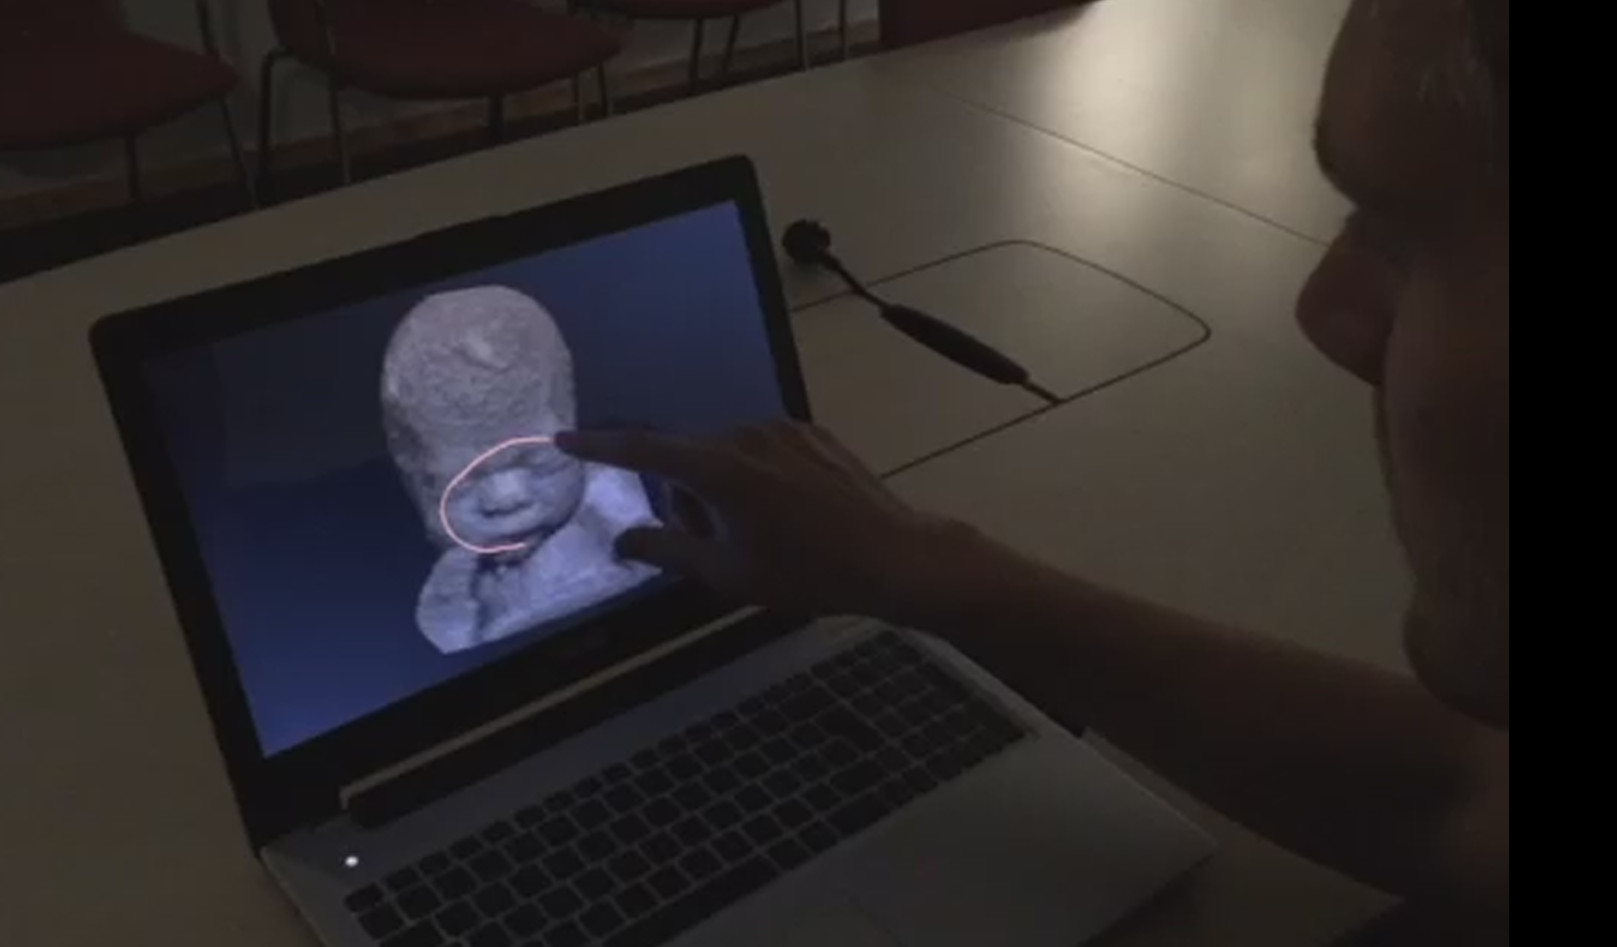
\includegraphics[width=1.0\linewidth]{images/touch_workstation}}
	\caption{Visualization of a fetus scanned using ultrasound. Touch screen interaction is used to change parameters such as camera, transfer function and clipping.}
	\label{img:touch_workstation}
\end{figure}

\begin{figure}[t]
	\centering
	\fbox{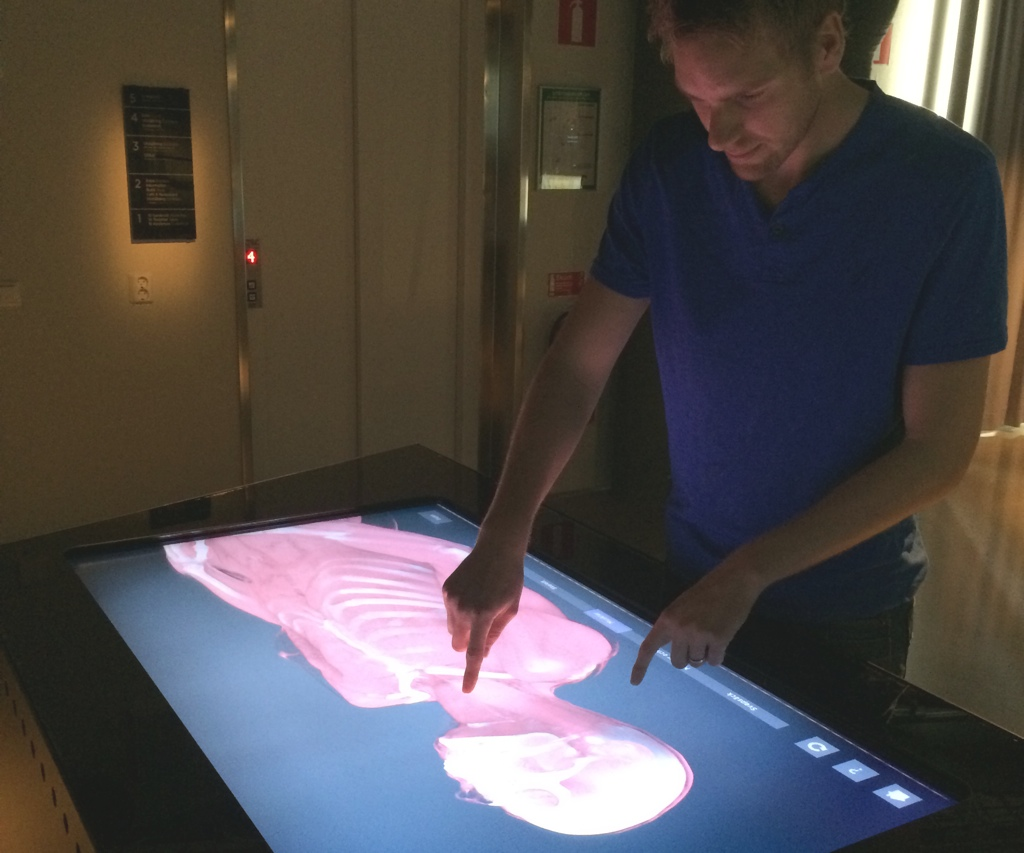
\includegraphics[width=1.0\linewidth]{images/exhib_table}}
	\caption{A touch table (known as the Virtual Autopsy Table) for presentation of, for instance, CT scanned medical data.}
	\label{img:exhibition_table}
\end{figure}

\subsection{Presentations in Exhibition Area} \label{sec:exhibition}
In a public exhibition area, both small to medium sized displays are often utilized to showcase and explore scientific data.
It is mostly targeted at non-expert users and viewers that interact, and see others interact, which requires intuitive and natural input methods.
There exist a wide range of setups with displays and gadgets for immersive and exploratory purposes that can be utilized in an exhibition area~\cite{Laha:2013:VCB:2491367.2491368, conf/egve/KruszynskiL08}.
That fact, together with a reasonable level of functionality, motivates the usage of a hands-only setup either through direct touch~\cite{Klein:2012:DSD:2322389.2322403} or touchless methods~\cite{O'hara:2013:NTP:2442106.2442111}.

Figure~\ref{img:exhibition_table} shows an exhibition setup example, known as the virtual autopsy table~\cite{LRFPY11}, where data, such as a CT scan of a human, can be explored using multi-touch gestures.
Rotation and translation of the object are done via vertical and horizontal movements, while zooming is performed with a two-finger pinch gesture.
Various 2D icons are shown around the visualization for state switching and presenting relevant information about the data.
Other icons are used to change clipping and transparency levels within the visualization, which are also manipulated with a single finger touch.

Although the table works basically the same as a handheld device, it is more appropriate for a larger audience as the area surrounding the table increases the accessibility to both the interaction surface and the visualization.
This type of setup has been appreciated by both the presenter and the audience due to intuitive interaction as well as the large display.
%However, the larger the touch display surface is, the more the presenter has to move, which puts size constraints on these devices.

%Limiting the interaction to touch gestures can be a challenge as there is a 2D input for a 3D environment.
%However, interaction with touch displays is so widely adopted that a gesture language has been developed using common gestures such as pinch and swipe.

The setup in Figure~\ref{img:exhibition_kinect} can, at a first glance, seem similar to Figure~\ref{img:exhibition_table} in terms of exploring data.
However, the display surface does not have direct touch capabilities, but is controlled by tracking the movements of the presenter's hands in 3D.
The visualization is supported by state icons, which allow the presenter to select a data set from a choice of four presets.
A hand cursor is rendered onto the screen that mimics the movements of the presenter's right hand.
The left hand is tracked and utilized to switch between different rendering states such as moving the camera or light source interaction.

\begin{figure}[tb]
	\centering
	\fbox{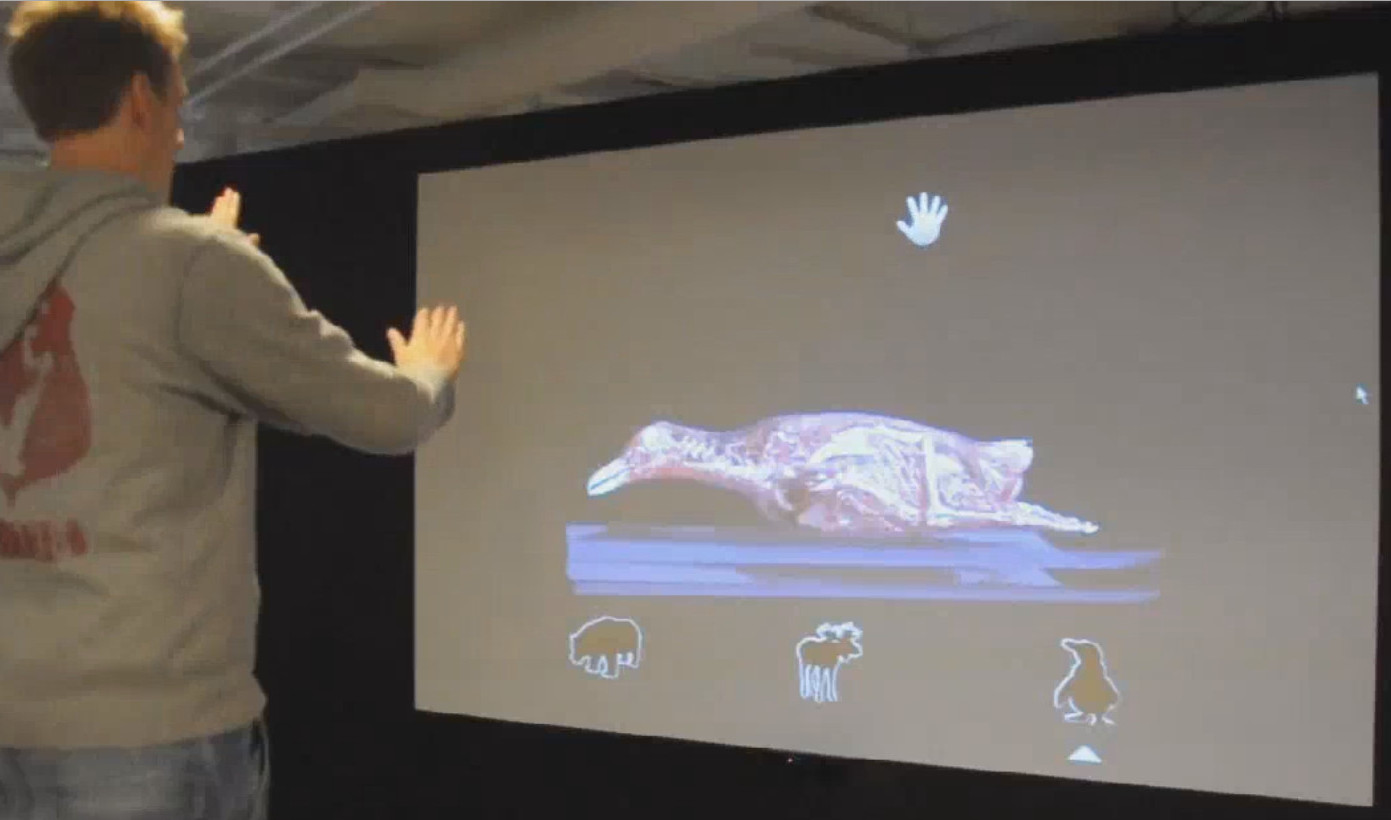
\includegraphics[width=1.0\linewidth]{images/exhib_rotate_peng}}
	\caption{Volume visualization of a CT scanned penguin displayed on a wall with a in-front projector and coupled with a kinect for 3D interaction possiblities.}
	\label{img:exhibition_kinect}
\end{figure}

\subsection{Presentations in an Auditorium} \label{sec:largeaudience}
A common scenario is a presenter standing in front of a seated, or otherwise stationary, audience. 
The audience is typically large, ranging from tens to hundreds of people.
The display system we use in this scenario is a wide field-of-view hemispherical dome surface with seating for 99 audience members (see Figures~\ref{img:dome_presentation} and~\ref{img:dome_clip}).
The dome theater is similar to traditional planetariums, but the content is produced using an interactive rendering system instead.
Due to the size of the screen, and large difference in seating location, it can be difficult for parts of the audience see both the visualization and the presenter at the same time. 
In addition to this, small movements may be hard to see for the audience in the back seats. 
The main interaction technique used by the presenter in practice is talking to an operator which, in turn, directly controls the visualization.
From the point of view of the audience the operator is completely transparent and the interaction ends with the presenter verbally giving commands.

We have also made experiments with touchless interaction, where gestures are performed though finger and hand movements, as seen in Figure~\ref{img:dome_clip}.
Here, movements are designed to reflect the operations performed on the screen.
For instance, moving a clip plane towards and away from the camera is done by the presenter moving his hands towards and away from himself. As the whole-body can be tracked in 3D the presenter could reach out to pull or push the visualization closer or further away.

%A slight variant to oral presentations is the concept of remote presentations.
%In this case, the presenter is not in the same room as the intended audience, but the voice (and possible video footage) is streamed instead.
%Regarding the interaction there is no difference as the presenter's interaction with the content is limited to communication and there is no physical input necessary.
%The only visible difference to the audience is the missing presence of the presenter in the same room, which might make other, complementary, sources of interaction impossible (such as using laser pointers).
%An increase in future presence technologies will eventually blur the line further between a physically-present presenter and a remote presenter.

%The third setup is a curved-screen decision arena in which the audience members are located on the inside of a round room with the walls being used as projection surfaces.
%This setup is very useful for a small group of people ($<$ 10 persons) to simultaneously work on decisions using the information projected on the surfaces.
%The interaction techniques for this, as compared to the previous two, are fairly limited in regular usage, as this is not a tradition presentation setup, but rather a collaborative exploration of data using visualization.



%Presenter is always decoupled from the screen, as the presenter can not interact with the complete presentation surface. This is often due to the lack of touch capability, but foremost the sheer size of common screens for large audience presentations can not be reached from a standing location by the user.

%Dome, movement, viewers benefit to see how presenter interacts with the data.
%Thus, big 3D gestures better then gesture on touch device.

%User should be standing in such away that the 3D movements the user performs can be projected correctly onto the screen.

%Discuss interaction option made by audience, pros and cons

%\begin{figure}[htb]
%	\centering
%	\fbox{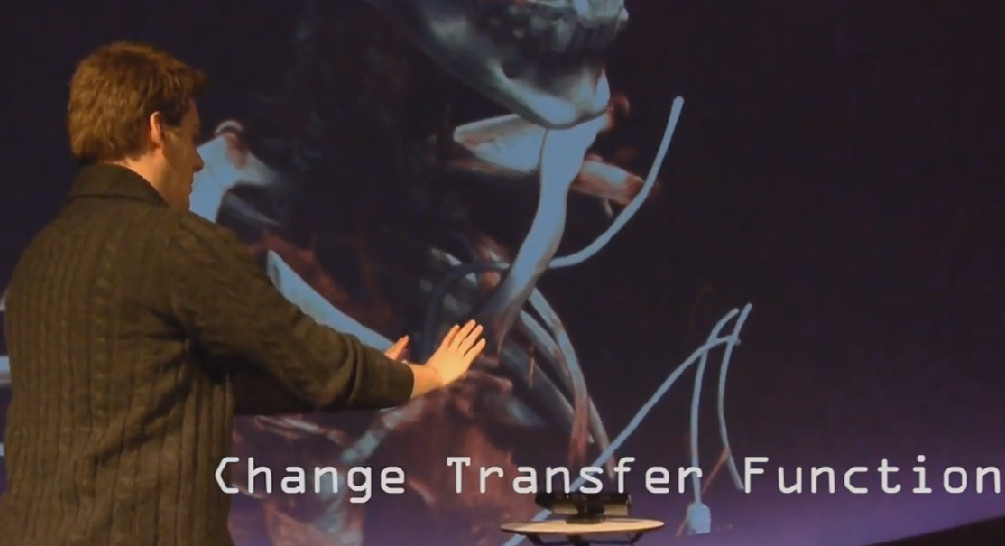
\includegraphics[width=1.0\linewidth]{images/dome_tf_change}}
%	\caption{Dome Closeup}
%	\label{img:dome_tf_change}
%\end{figure}

\begin{figure}[t]
	\centering
	\fbox{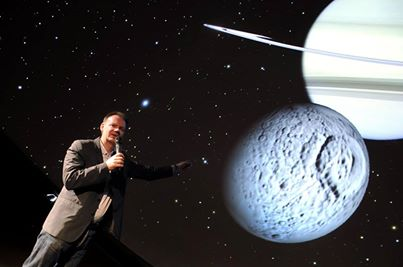
\includegraphics[width=\linewidth, height=165pt]{images/dome_oralpresentation}}
	\caption{Presentation on large scale surface using the voice as an interaction technique to communicate intent rather than direct instructions.}
	\label{img:dome_presentation}
\end{figure}

\section{Interaction techniques from the scenarios} \label{sec:techniques}
The purpose of this paper is not to cover every possible interaction setup best suited for the scenarios, but rather to analyze the current ones and categorize them in different groups that are utilized throughout the scenarios.
Therefore, we summarize the interaction techniques that can be derived from of our scenarios and discuss their applicability.

\subsection{Direct Touch Interaction}
Direct interaction with an object in the scene gives the user a feel of control over the object~\cite{isenberg2009studying}. 
The user touches the screen and the 2D motion is mapped to a 3D manipulation of the object, for instance by mimicking the interaction of a trackball.
In scientific visualization, touch interaction has not received much attention in the past \cite{isenberg:hal-00781512}, but more work is starting to appear~\cite{Klein:2012:DSD:2322389.2322403} and it has already been used in applications~\cite{LRFPY11}.
This type of interaction is present in Scenarios \ref{sec:workstation} and \ref{sec:exhibition}, where differently sized touch screens are utilized. 
When analyzing this interaction technique from a presentation perspective, the audience can see the movements of the presenters' hands and fingers and, through that, get an understanding of what will happen on the display device.
Furthermore, there is little distance between the interaction plane and the display surface and, thus, spatially correlated interaction events are well perceived.
However, the presenter hides part of the screen due to the occluding hands and arms.
Thus, when the audience grows larger it becomes harder for every audience member to see the gestures.
This type of interaction is not present in Scenario \ref{sec:largeaudience}, where both the audience and the presenter are at a physical distance from the projection surface.
The dome presentation scenario makes direct techniques, such as pointing with a finger or performing gestures that are directly related to the content's position on the screen difficult mainly due to the large distance between the presenter and the screen.
Instead, indirect techniques must be used such as laser pointers, rendered cursors on the screen, gesture recognition or verbal communication.

\begin{figure}[htb]
	\centering
	\fbox{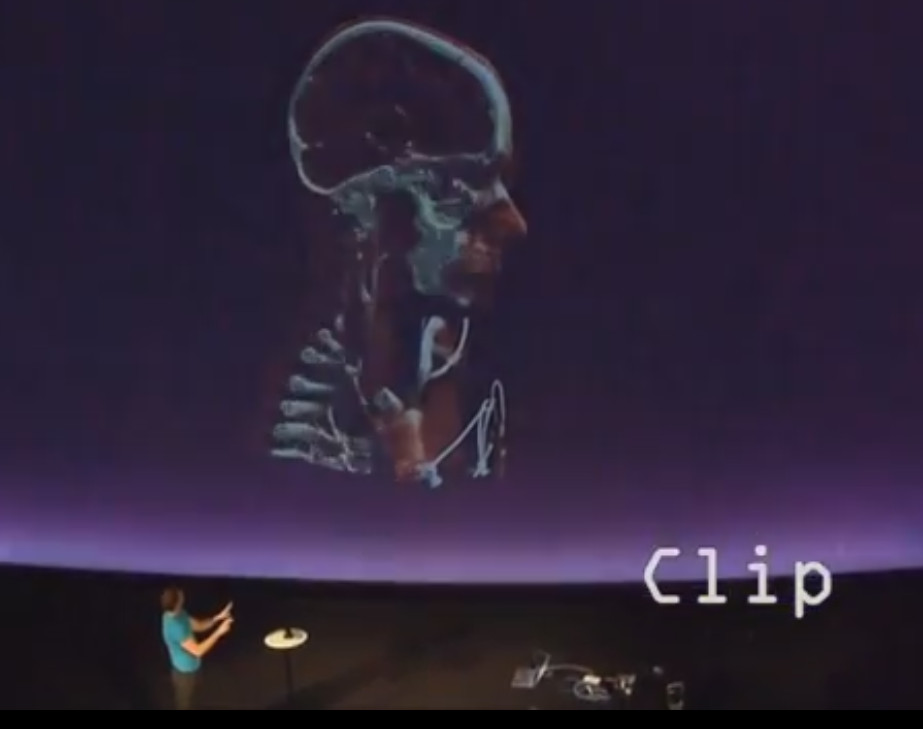
\includegraphics[width=1.0\linewidth]{images/dome_clip}}
	\caption{Presentation on large scale surface using the kinect device as an interaction technique to interact with the visualization trough hand gestures.}
	\label{img:dome_clip}
\end{figure}

%Importance of Touch \cite{Robles-De-La-Torre:2006:IST:1158827.1159097}

\begin{figure*}
    \centering
    \subfigure[The figure shows which interaction technique category that is applicable for varying audience sizes and display sizes. The ordering does not imply any judgement on preference of one method over another. Voice control is applicable everywhere.]{
        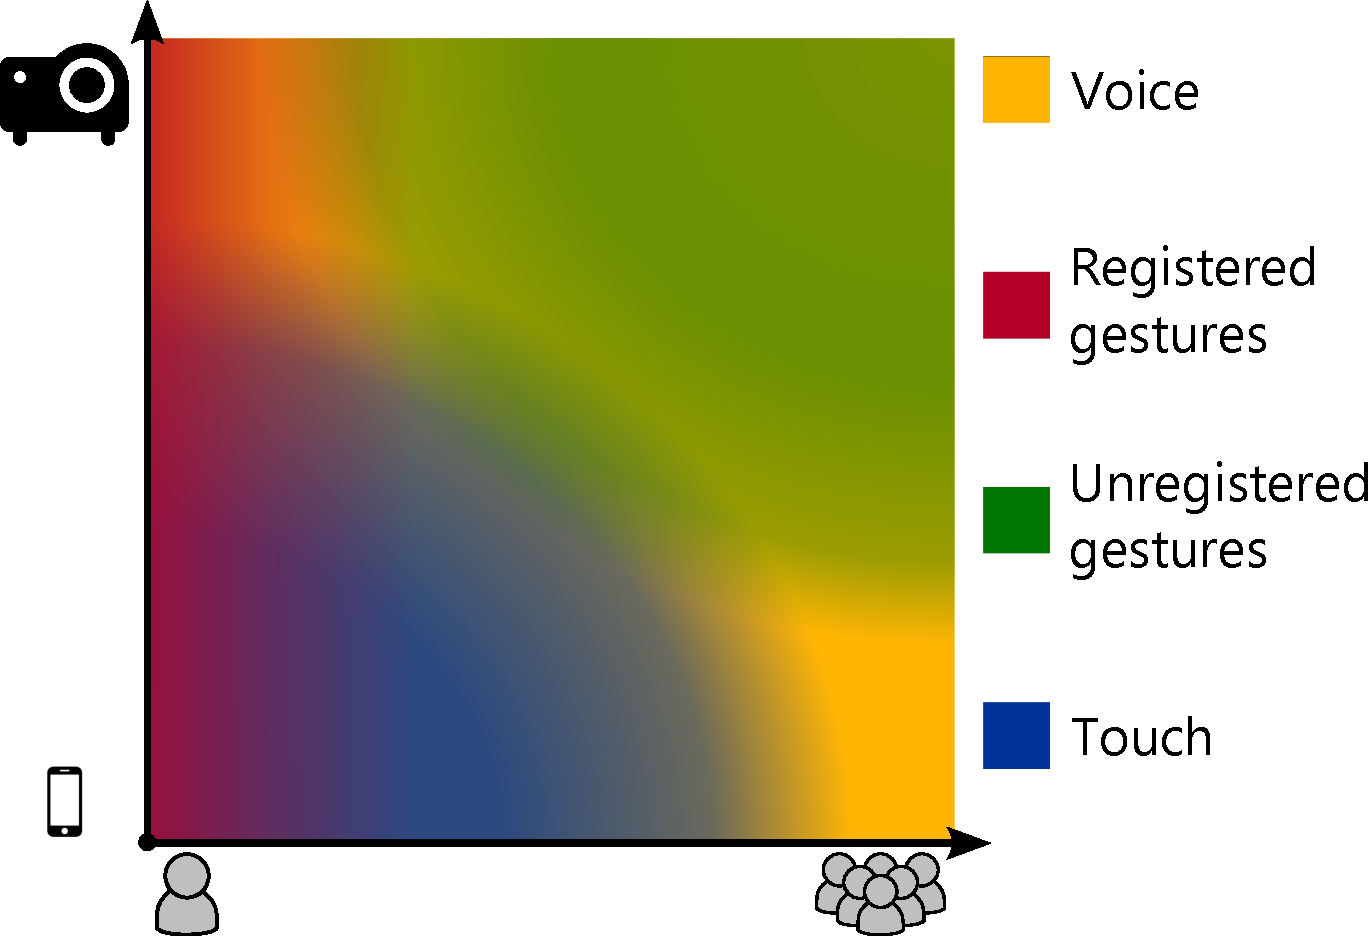
\includegraphics[height=0.65\columnwidth]{classification.pdf}
        \label{classifiy_diagram}
    }
    \hfill
    \subfigure[Showing to which audience sizes and display sizes the scenarios described in Section~\ref{sec:scenario} are relevant.]{
        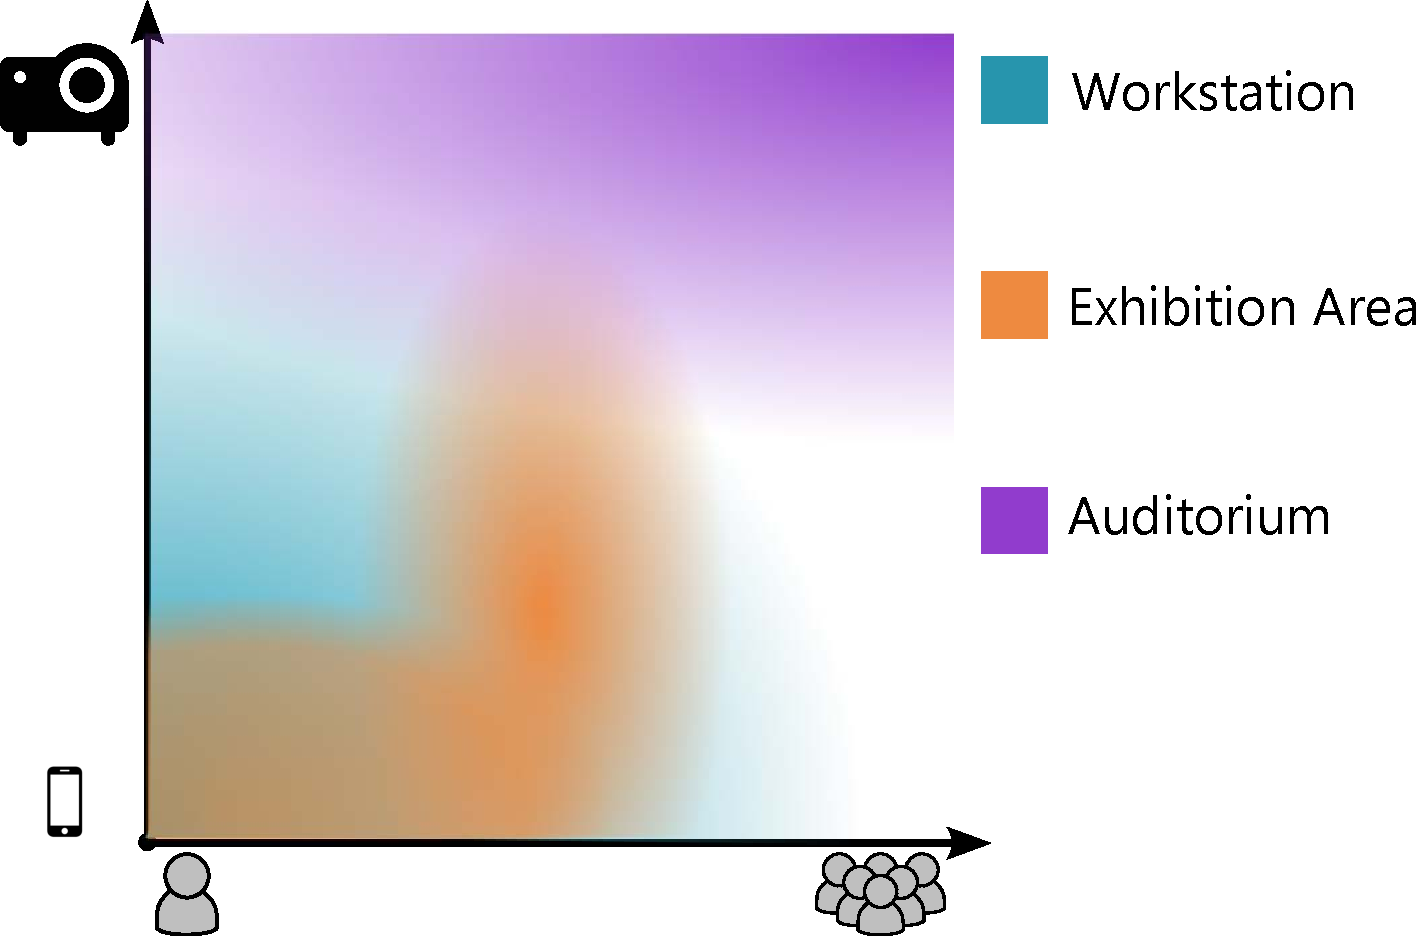
\includegraphics[height=0.65\columnwidth]{expressivity.pdf}
        \label{scenario_diagram}
    }
		\caption{Showing the applicability and relevance of different interaction types and various environments. By using a side-by-side comparison of the two figures, it is possible for interaction designers to pick a good subset of interaction techniques (a) for a specific scenario (b).}
		\label{our_charts}
\end{figure*}

\subsection{Touchless Interaction}\label{subsec:touchless}
Touchless interaction is useful in situations, such as surgery~\cite{Mentis:2012:IPI:2207676.2208536}, where touching an interaction device is cumbersome or must be avoided due to, for example, hygienic constraints.
Moving hands freely in the air enables expressive gestures without being restricted to 2D motion as in the case of direct touch interaction.
However, recognizing the start and end point of a gesture can be difficult since there is no natural deactivation state~\cite{Kirmizibayrak:2011:EGB:2087756.2087764}.
Furthermore, the presenter might feel less in control of the data, even neglecting the accuracy of the tracking, as the person is not directly touching the display surface.
However, the movements are often expressive and can therefore be seen more clearly by the audience during a presentation.

Our Scenario~\ref{sec:exhibition} includes both a direct touch and a touchless setup, and both setups have been used interactively when presenting scientific data for the same group, usually consisting of around 10-20 people.
The touchless setup can support a larger audience due the placement of the display surface, but has the downside of a decoupled interaction experience, where the interaction is performed farther away from the display surface.

As we evaluate the interaction from an presentation perspective and how the audience perceive it, we have divided touchless interactions into two categories; registered and unregistered gestures.
We refer to an \emph{unregistered gesture} when the audience sees that the presenter is performing interactions that are clearly decoupled from the display. 
A \emph{registered gesture} could be touchless if the audience perceives it as performed in correlation of the display surface, such as interactions close to a wall-sized displays, as detailed in~\cite{Bezerianos:2007:DSU:1467769}, which is also the fact with all gestures on a touch screen. 
For instance, a few number of people standing behind the presenter can see the presenters hands and how they are projected on the display, even if the presenter is standing far away from the display.
Thus, when utilizing the correlation between the hand positions and the display, they are registered gestures even if there is a touchless setup.
With this distinction in mind, most of the audience in the touchless setup in Scenario~\ref{sec:exhibition} will see the gestures performed by the presenter as unregistered gestures, while only a few might look upon it as registered gestures.
In a presentation sense, we prefer registered gestures over unregistered gestures, as the audience may benefit from interaction which is closely correlated with the content.
 
When a decoupled interaction approach is necessary, certain elements can be introduced in order to help the audience.
As seen in Figure~\ref{img:exhibition_kinect}, a hand cursor is rendered that simulates the projection of the presenter's hand on the surface.
Such visual cues not only help the presenter, but also allow the audience to better comprehend which operation the presenter is currently performing, as they can correlate the location of the presenter's hand in relation to the display.
Furthermore, the icons in the bottom of the screen do not only avoid an increase in the number of necessary gestures, but also to make the operations performed relate more directly to the visualization. 
When the presenter is moving the hand towards an icon, the audience might perceive that the action is about to happen as compared to performing the same operation through a gesture or posture~\cite{isenberg:hal-00781237}. 
Thus, whole body movements \cite{978-0-85729-432-6, Shoemaker:2010:BIT:1868914.1868967} might increase how well the audience perceives what the interaction is altering in the visualization even further.

This type of interaction is also present in Scenario~\ref{sec:largeaudience}. The type of touchless interaction setup is quite similar, however both the audience size and the display size are substantially increased.
One issue with this system is the difficulty in mapping physical gestures to match the visualizations due to the large scale of the room and the large differences in seating position.
It is not possible to place the presenter in such a way that the gestures would seem integrated into the visualization for all viewers simultaneously.

Seen from an audience's perspective the touchless gestures in this setup are more expressive than what direct touch gestures on a handheld device or a touch table would be.
Thus, the touchless setup could be considered as a more expressive presentation tool than utilizing a touch device for remote communication, as done by Coffey~\textit{et al.}~\cite{Coffey:2012:ISW:2360744.2360843}.

%Touching the 3rd dimension \cite{DBLP:journals/dagstuhl-reports/KeefeKSR12}

%Evaluation of Gesture \cite{Kirmizibayrak:2011:EGB:2087756.2087764}

%Discuss gesture vs postures \cite{isenberg:hal-00781237} for kinect, and gesture available for both touch and kinect.

%Mouse vs Kinect vs Leap vs Myo \cite{doi:10.1117/12.2006994}. \todo{I would like to see a paragraph somewhere saying that the actual technology does not matter for the interaction, as there is no big difference between a kinect or a leap motion, for example. (ab)}

\subsection{Voice Control}

Interacting with the visualization by voice is performed in scenario~\ref{sec:largeaudience} (see Figure~\ref{img:dome_presentation}), where the presenter is communicating verbally with an entity controlling the visualization.
The voice acts as an input itself and becomes an interface device between the presenter and the content.
For our argumentation, there is no difference if the presenter is communicating with an operator steering the visualization, or an advanced voice-recognition system, as the audience does not know how the verbal commands are processed.
%From the audience's point of view, the presenter is the user of the system and the voice is the interaction technique, and the audience does not know (or care) what happens afterwards.
%
%From an interaction point of view, this interplay between presenter and controller has both benefits and drawbacks.
%One benefit is the dynamics between the presenter and the controller, creating a more engaging environment for the audience, itself sparking more interaction between the audience and the presenter.
From an interaction point of view, this means that the audience is witness to the intended action of the interaction, rather than the physical act of interacting itself.
The audience knows that, for example, the focus will be on a specific part of a rendering before it happens.
Rather than witnessing the manual interaction leading to that focus, it perceives the interaction as being completely decoupled from the presenter.
By removing any signs of a physical interaction, the presenter can focus on the explanations and content rather than multitasking with the presentation and the controlling.

In a presentation aspect, this interaction could generally be perceived as very expressive and beneficial as the audience can understand directly what is going to happen trough the voice command, before it happens, if there is a natural correlation between the command and the changes performed in the visualization.
However, even for a perfect voice interaction system, the ambiguity of natural language can require a long-winded explanation in cases where precise interaction is needed. Another downside is that the presenter must interrupt the presentation to give commands and there might also be a time delay before the command is executed.

\section{Classification} \label{sec:classification}

In order to show the applicability of an interaction technique for the audience, we introduce a classification of the techniques covered in our scenarios.
Figure~\ref{classifiy_diagram} shows where the techniques are applicable in relation to audience size and display size. 
We chose to split up the touchless interaction in our scenarios into registered and unregistered gestures, as previously detailed in Section \ref{subsec:touchless}.

The conclusion which can be drawn from our mapping is that in our scenarios, direct touch is utilized for interaction using small to medium-sized displays with a small to medium-sized audience. 
Furthermore, registered gestures, where the presenters interaction is correlated with the visualization and the display, are utilized for all display sizes, but only for an audience of very few people.
Unregistered gestures are utilized when the display area and audience size is large, as not all people from the audience would be able to see the presenter's interaction, or when the display surface is too large for close interaction.
Voice control could be used in most variations of display and audience sizes. However, we reckon that this interaction might be most preferable when no other technique is suitable since current technology does not allow enough complex and flexible interaction.

In Figure~\ref{scenario_diagram} we complement Figure~\ref{classifiy_diagram} such that a mapping between our techniques and our scenarios can 
be performed using a side-by-side comparison.

Our classifications are introduced with the purpose of not only showing the status quo, but also for supporting the selection of interaction techniques for future presentation scenarios, with the use of parameters such as audience size and display.

There are more advanced classification methods for interaction techniques~\cite{stars:65-93:2012}, especially for 3D user interaction~\cite{978-3-319-07458-0_1, CGF:CGF194, Kettner95aclassification}, but the focus of these classifications is on the usability from a user perceptive only, rather than the applicability in presentation scenarios.

\section{Conclusions}\label{sec:conclusion}

In this paper we share our thoughts, observations and experiences about interaction techniques in visualization from an audience-centric view, rather than the more common user-centric exploratory way of designing and evaluating appropriate interaction methods.

In the previous sections, we described presentation scenarios that require interaction and we examined the types of interaction utilized today, such as 2D/3D user interfaces and voice.
Although it would be interesting to include interaction techniques that involves hand-held devices it was not the focus in this work.
In the same aspect not all scenarios where interaction might be suitable is covered.
Such an evaluation would be extensive and beyond the scope of a position paper.
Furthermore, new types of interaction techniques and usage scenarios can be put into context using Figure~\ref{our_charts}, thereby giving initial directions on suitable combinations of new interaction techniques and scenarios.

We deem that research within audience-centered interaction techniques should receive more attention as these are an essential part of the visualization, knowledge-transfer and communication. 
We strongly encourage researchers developing 2D and 3D user interaction interfaces to include this aspect when evaluating previous and future techniques.
Within this subject, expert and non-expert viewers have different experiences with scientific data and interaction techniques. Thus, the naturalness of the interaction could therefore be completely different for various group of viewers.
\bibliographystyle{abbrv}
%%use following if all content of bibtex file should be shown
%\nocite{*}
\bibliography{literature}
\end{document}
